\documentclass[12pt, a4paper]{article}
\usepackage[margin=1.25in]{geometry}
\usepackage{graphicx}
\usepackage{amsmath}
\usepackage{float}
\usepackage{listings}
\usepackage{caption}
\usepackage{physics}
\usepackage[shortlabels]{enumitem}


\setlength\parindent{0pt}
\newcommand{\code}{\lstinline[basicstyle=\small]}
\lstset{
    language=Python,
    basicstyle=\scriptsize
}


\title{EE2703: Applied Programming Lab \\ \Large Assignment 7: Circuit Analysis using Sympy}
\author{Soham Roy \\ \normalsize EE20B130}
\date{\today}
\begin{document}

\maketitle % Insert the title, author and date



\section{Introduction}
The goal of this assignment is to understand the symbolic algebra capabilities of python and to circuits using
the Laplace Transform. \\
The aim is also to understand the basics of the high pass and low pass filter circuits.



\section{Subquestions}
\subsection{Question 1}
To find the transfer function of the given circuit, and then find the unit step response.
Solving the circuit by using the basic KCL and KVL laws, we get the following solution in matrix form:
\[
    \begin{pmatrix}
        0                                    & 0             & 1 & -1/G \\
        \frac{-1}{1+sc_2R_2}                 & 1             & 0 & 0    \\
        0                                    & -G            & G & 1    \\
        -\frac{1}{R_1} -\frac{1}{R_2} - sC_1 & \frac{1}{R_2} & 0 & sC_1
    \end{pmatrix}
    \begin{pmatrix}
        V1 \\
        Vp \\
        Vm \\
        V0
    \end{pmatrix}
    =
    \begin{pmatrix}
        0 \\
        0 \\
        0 \\
        -\frac{Vi(s)}{R_1}
    \end{pmatrix}
\]

We then use the \code{sympy} library to implement this in python and also solve for the voltage vector.
We calculate the Voltage response for a unit input, which would thus give me the transfer function of this circuit.
We then plot the Frequency response of this circuit. The following is the code:

\begin{lstlisting}
    def lowpass(Vi, R1=10000, R2=10000, C1=1e-9, C2=1e-9, G=1.586):
        A = sym.Matrix(
            [
                [0, 0, 1, -1 / G],
                [-1 / (1 + s * R2 * C2), 1, 0, 0],
                [0, -G, G, 1],
                [-1 / R1 - 1 / R2 - s * C1, 1 / R2, 0, s * C1],
            ]
        )
        b = sym.Matrix([0, 0, 0, -Vi / R1])
        V = A.inv() * b

        return A, b, V

        
    title = "Lowpass Filter Magnitude Response"

    A, b, V = lowpass(1)
    V_o = V[3]
    print(V_o)
    ww = np.logspace(0, 8, 801)
    ss = 1j * ww
    H = sym.lambdify(s, V_o, "numpy")
    HH = H(ss)
    plot(title, "$\omega (rad/s)$", "$|H(j\omega)|$",
         ww, [abs(HH)], plotting_fn=plt.loglog)
\end{lstlisting}
The following plot is obtained.

\begin{figure}[H]
    \centering
    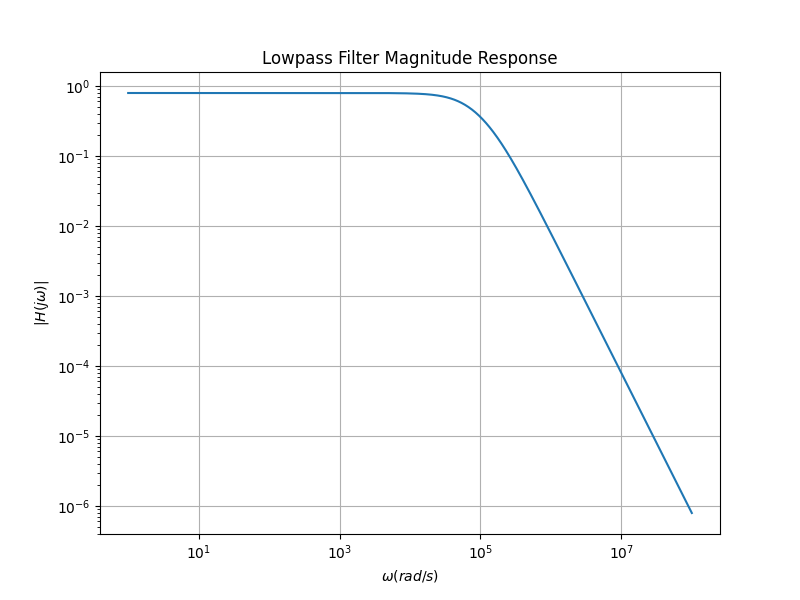
\includegraphics[scale=0.6]{0.png}
\end{figure}

Once we have obtained the system response in \code{sympy} symbolic form, we need to convert it to our standard
\code{scipy.signal.lti} form in order to work with it further, the following function does this job.

\begin{lstlisting}
    def to_num_den(expr):
        num, den = expr.as_numer_denom()
        num = [float(i) for i in sym.Poly(num, s).all_coeffs()]
        den = [float(i) for i in sym.Poly(den, s).all_coeffs()]
        return num, den
\end{lstlisting}

The unit step response of the circuit i.e the output for an input of $u(t)$ is calculated using the following code:

\begin{lstlisting}
    title = "Lowpass Filter Step Response"

    V_o = lowpass(1 / s)[2][3]
    H = sp.lti(*to_num_den(V_o))
    t = np.linspace(0, 5e-3, 10000)
    v = sp.impulse(H, T=t)[1]
    plot(title, "$t (s)$", "$V_o (V)$", t, [v])
\end{lstlisting}

The following plot is obtained:
\begin{figure}[H]
    \centering
    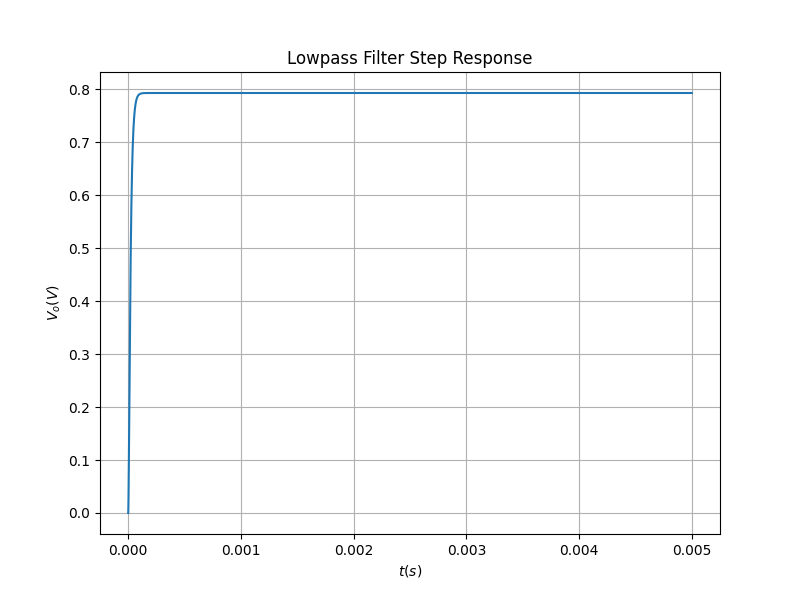
\includegraphics[scale=0.6]{1.png}
\end{figure}

\subsection{Question 2}
This time, we need to obtain the output for a mixed frequency input
\[V_i(t) = (\sin(2000\pi t)+\cos(2*10^6\pi t))u_0(t) Volts\]

This is done as follows:
\begin{lstlisting}
    title = "Lowpass Filter Input Response"

    V_o = lowpass(1)[2][3]
    H = sp.lti(*to_num_den(V_o))
    t = np.linspace(0, 5e-3, 100000)
    input = (np.sin(2000 * np.pi * t) + np.cos(2e6 * np.pi * t)) * (t > 0)
    v = sp.lsim(H, U=input, T=t)[1]
    plot(title, "$t (s)$", "$V (V)$", t, [input, v], ["Input", "Output"])
\end{lstlisting}

The following plots are obtained:
\begin{figure}[H]
    \centering
    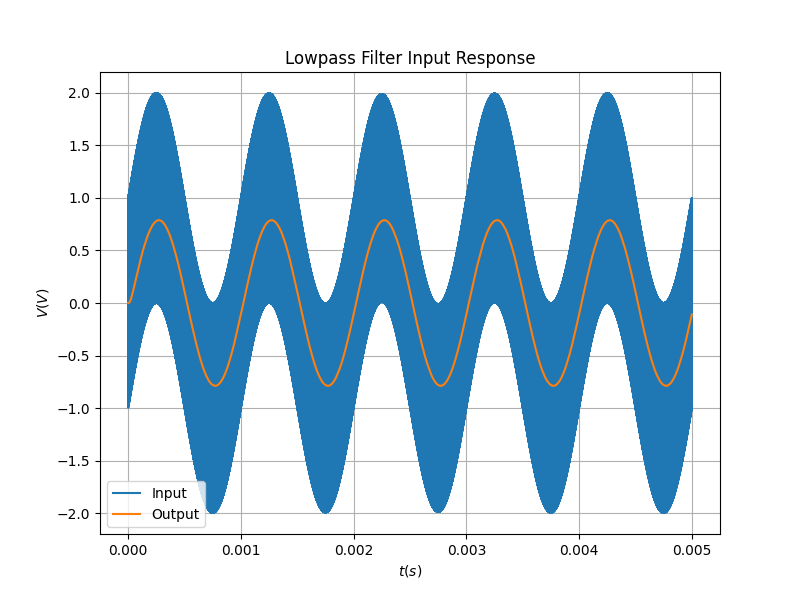
\includegraphics[scale=0.6]{2.png}
\end{figure}

This can be explained easily, since we know that a low pass filter only allows those frequencies to pass which are less than the pole frequency, i.e in this case $10^5$, thus the $10^3$ frequency component passes, whereas the $10^6$ frequency component is filtered out. \\Due to the very high frequency of the $10^6$ frequency signal, it appears as if this signal oscillates about the $10^3$ frequncy signal with the latter as it's mean value, in the input.

\subsection{Question 3}
Now, we try to do the same analysis for a high pass filter. A high-pass filter is a filter that passes signals with a frequency higher than a certain cutoff frequency and attenuates signals with frequencies lower than the cutoff frequency.
The code for this part is as follows:
\begin{lstlisting}
    def highpass(Vi, R1=10000, R3=10000, C1=1e-9, C2=1e-9, G=1.586):
        A = sym.Matrix(
            [
                [0, -1, 0, 1 / G],
                [s * C2 * R3 / (s * C2 * R3 + 1), 0, -1, 0],
                [0, G, -G, 1],
                [-s * C2 - 1 / R1 - s * C1, 0, s * C2, 1 / R1],
            ]
        )
        b = sym.Matrix([0, 0, 0, -Vi * s * C1])
        V = A.inv() * b

        return A, b, V


    title = "Highpass Filter Magnitude Response"

    A, b, V = highpass(1)
    V_o = V[3]
    print(V_o)
    ww = np.logspace(0, 8, 801)
    ss = 1j * ww
    H = sym.lambdify(s, V_o, "numpy")
    HH = H(ss)
    plot(title, "$\omega (rad/s)$", "$|H(j\omega)|$",
         ww, [abs(HH)], plotting_fn=plt.loglog)   
\end{lstlisting}

The following is the frequency response for the given high pass filter:

\begin{figure}[H]
    \centering
    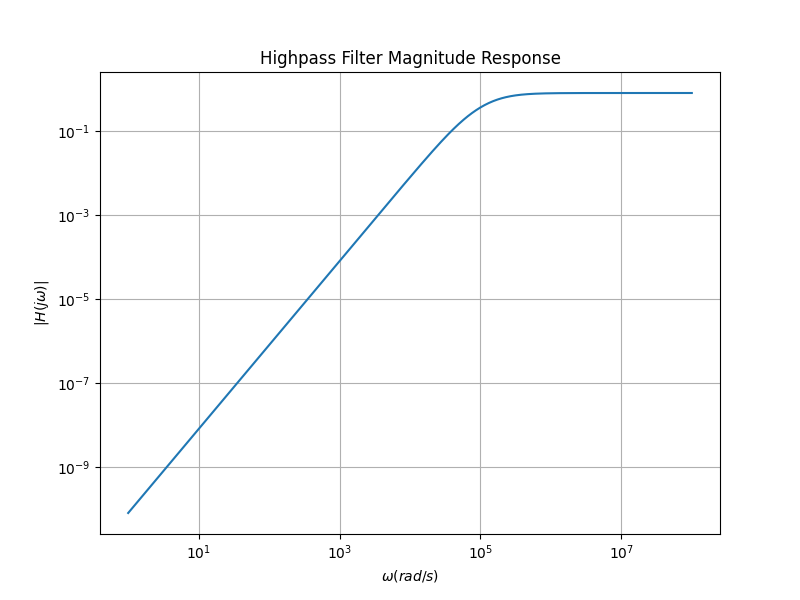
\includegraphics[scale=0.6]{3.png}
\end{figure}

\subsection{Question 4}
Now, we try to obtain the response of this filter for a damped sinusoidal input as follows:
\[V_{i, hf}(t) = e^{-5 \cdot 10^4t} cos(2\pi \cdot 10^8 \cdot t) \]
\[V_{i, lf}(t) = e^{-5t} cos(2\pi \cdot 10 \cdot t)\]

The code for this is as follows:
\begin{lstlisting}
    title = "Highpass Damped Response for High Frequency"

    V_o = highpass(1)[2][3]
    H = sp.lti(*to_num_den(V_o))
    t = np.linspace(0, 1e-4, 1000)
    input = np.cos(2 * np.pi * 1e8 * t) * np.exp(-5e4 * t) * (t > 0)
    v = sp.lsim(H, U=input, T=t)[1]
    plot(title, "$t (s)$", "$V (V)$", t, [input, v], ["Input", "Output"])
    
    
    title = "Highpass Damped Response for Low Frequency"
    
    t = np.linspace(0, 1, 1000)
    input = np.cos(20 * np.pi * t) * np.exp(-5 * t) * (t > 0)
    v = sp.lsim(H, U=input, T=t)[1]
    plot(title, "$t (s)$", "$V (V)$", t, [input, v], ["Input", "Output"])
\end{lstlisting}

The following graphs are obtained for the high frequency and low frequency inputs respectively.

\begin{figure}[H]
    \centering
    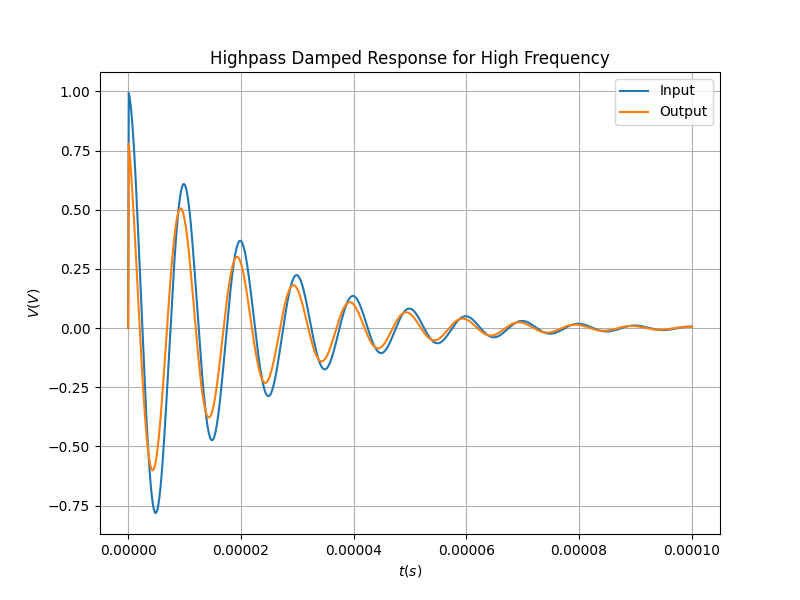
\includegraphics[scale=0.6]{4a.png}
\end{figure}

\begin{figure}[H]
    \centering
    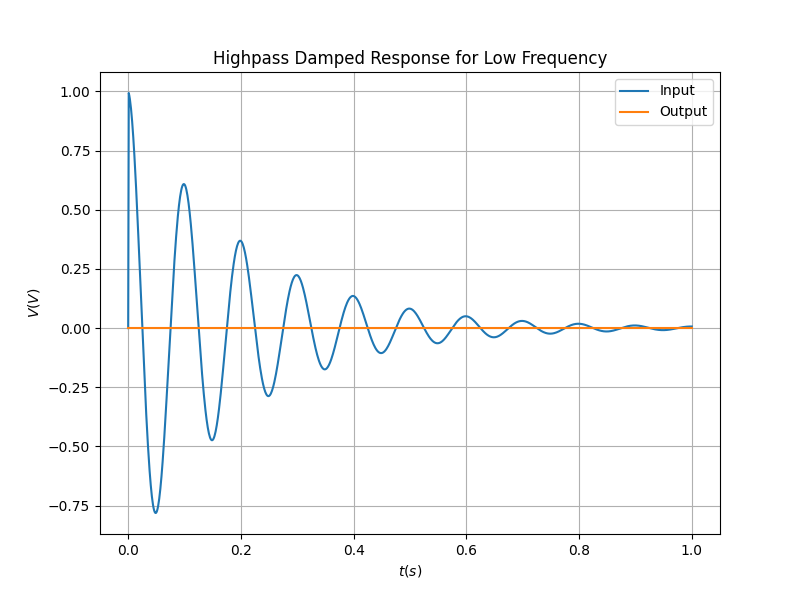
\includegraphics[scale=0.6]{4b.png}
\end{figure}

This can be explained quite easily, we know that a high pass filter will not allow the frequency components lower than pole freuqency to pass. Thus, effectively the low frequency component is filtered and thus it is not observed in the output.\\
Whereas, in the high frequency input case, we see that the output is pretty much same as the input, which indicates that our filter is working as required.

\subsection{Question 5}
We aim to find the unit step response of the high pass filter. For this, we pass $u(t)$ (in Laplace domain 1/s) in the \code{highpass} function, and then compute the inverse Laplace using the \code{scipy.signal.impulse} function.
The following code does this:

\begin{lstlisting}
    title = "Highpass Step Response"

    V_o = highpass(1 / s)[2][3]
    H = sp.lti(*to_num_den(V_o))
    t = np.linspace(0, 5e-3, 10000)
    v = sp.impulse(H, T=t)[1]
    plot(title, "$t (s)$", "$V_o (V)$", t, [v])
\end{lstlisting}

The following is the obtained response:
\begin{figure}[H]
    \centering
    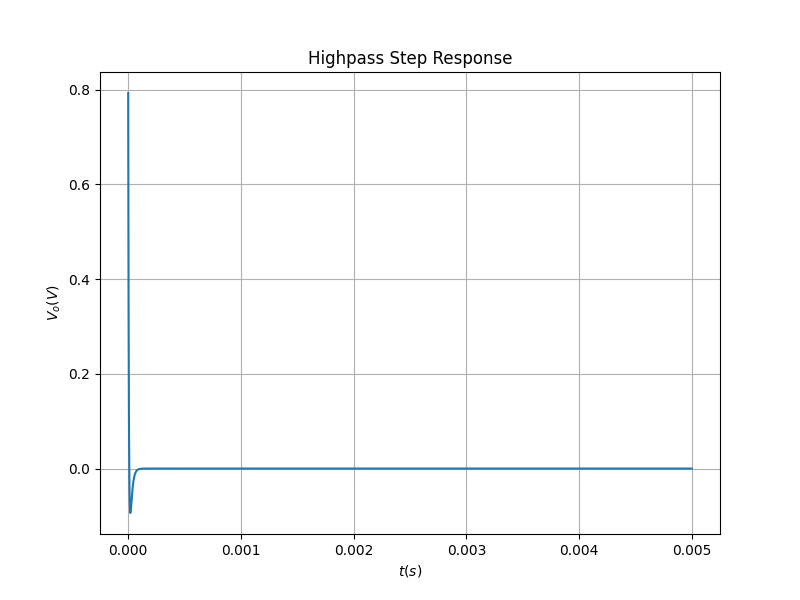
\includegraphics[scale=0.6]{5.png}
\end{figure}

Let's understand this response. As soon as the voltage is applied, i.e at t $\rightarrow0^+$, the capacitors behave as short-circuited, and thus we see a positive voltage at the output node, whereas at t $\rightarrow\infty$ (for practical purposes, this time is not that large), the capacitors would behave as open-circuited for DC-value of voltage and thus we would see zero volts at the output node.

\section{Conclusion}
In this assignment, we have understood the use of \code{sympy} library to do symbolic algebra. We have also learnt how this can be integrated with out previous knowledge of \code{scipy.signal} library to help solve circuits. We have also looked at some basic circuits like the high pass and the low pass filter and their responses for various inputs.


\end{document}
